\documentclass[12pt]{article}
\usepackage[margin=2cm]{geometry}
\usepackage{graphicx}
\usepackage{longtable}

\title{Are temperatures of one year significantly correlated with successive years, across years in a given location?}

\author{Elin Falla\\ef16@ic.ac.uk}

\date{}

\begin{document}
	\maketitle
	
	\section{Introduction}
		This study aims to determine whether the temperature in a given year at a given location is significantly correlated to the year following it.
		
	\section{Materials and methods}
		This study was conducted using R (version 3.4.2). From a dataset (Appendix 1) with a temperature given for $n$ years ($n$ = 100) I calculated the correlation coefficient between $n$ - 1 pairs of years using the cor() function. Due to the fact that measurements of climatic variables in successive time-points in a time series are not independent, I was not able to use the standard p-value calculated by cor(). I instead repeated the calculation $i$ times ($i$ = 10000) with a random permutation of the dataset in order to get $i$ correlation coefficients. I then calculated what fraction of these correlation coefficients were greater than that of the original dataset in order to get an approximation of the p-value.

	\section{Results and discussion}
		Figure~\ref{fig:dataset} shows a summary of the dataset - the temperature in each year. The each year is strongly positively correlated with its successive years, as the correlation of the ordered dataset was well beyond the 95th percentile of the correlation coefficients of random permutations (correlation coefficient = 0.33, p = 0.0004) (Figure~\ref{fig:histogram}).
		
		However, although this makes clear that the correlation of temperatures successive years is much higher than the correlation of temperatures in random years, it does not mean that temperature in year $n$ is strongly correlated with temperature in year $n$ + 1. The correlation coefficient was 0.33, suggesting the temperature in year $n$ alone is not a good predictor of the temperature in year $n$ + 1, although it can give an indication. There are likely other factors determining the temperature in a given year other than the temperature of the previous years.
		
		
	\begin{figure}
		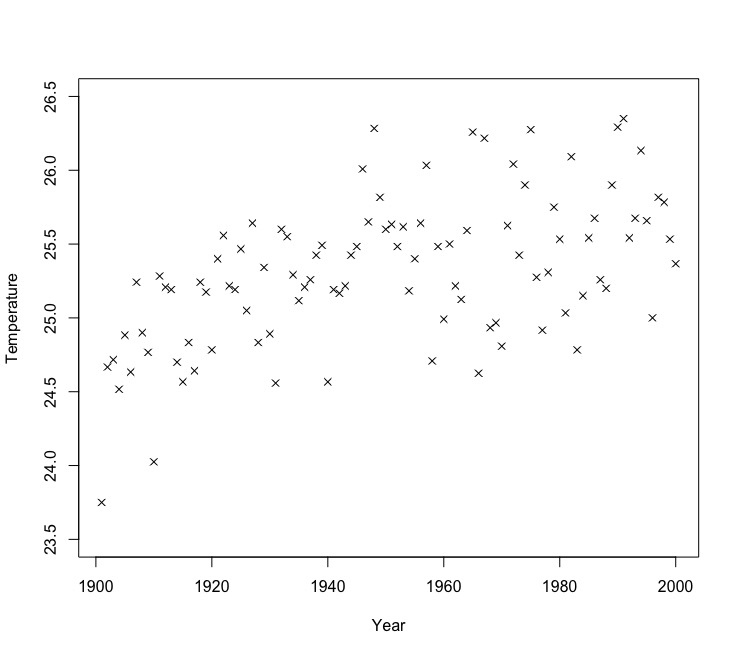
\includegraphics[width=\linewidth]{../Data/ats_yr_vs_temp.jpeg}				
		\caption{\label{fig:dataset} Temperature in each year of the dataset}
	\end{figure}
	
	\begin{figure}
		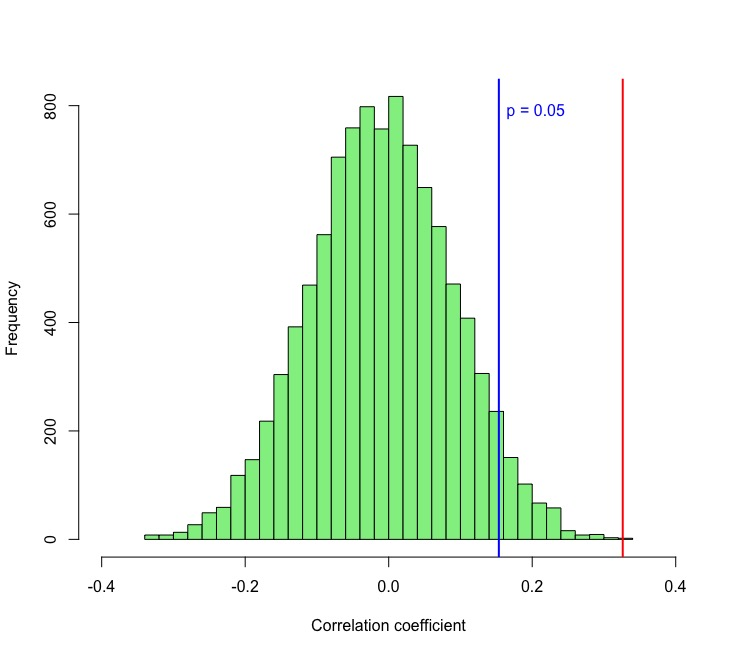
\includegraphics[width=\linewidth]{../Data/ats_corr_hist.jpeg}
		\caption{\label{fig:histogram} Frequency distribution of correlation coefficients for each of $i$ random permutations of the dataset. Blue line represents the 95th percentile of correlation coefficients (ie. p = 0.05). Red line represents correlation coefficient of true dataset (p = 0.0004). $i$ = 10000}
	\end{figure}
	
\end{document}